\subsection{Functional Requirements}

\subsubsection{Visitor scenarios}
\subsubsection*{Scenario 1}
Prabaker, a farmer from Telangana, wants to know how is the trend of agriculture in his country and for this reason he wants to have access to data about this. A friend of him, Sundar, suggested him to visit Dream’s web page, a project by the United Nations of India, giving him the link. Prabaker opens the link and connects to the site’s home page, where he can access different data set. Once he clicks on the button "Access the data" he notices that there’s the possibility to select different filters to see information coming from the various districts of Telangana. He decides to select the filter that shows how much rain has fallen in the last 24 hours in the zone of his land holding because in the monsoon season is important to keep track of it in order to not waste the crop. The page is rendered and he can see the updated data on screen.

\subsubsection*{Scenario 2}
Matteo, a researcher, needs to analyze soil quality data of the Telengana region about last month for his study in resource efficiency for crops in developing countries. He learns about project Dream that allows free access to all the resources he needs for his study. So Matteo connects to the Dream home page and then he selects the button to access the data. After doing that a new page is rendered and selecting a data set and scrolling down on it, he notices the possibility to download the data in different formats. He selects the one he suits the most and clicks on the button download.
\newpage

\subsubsection*{Use case diagram}
    \begin{figure}[hbt!]
        \centering
        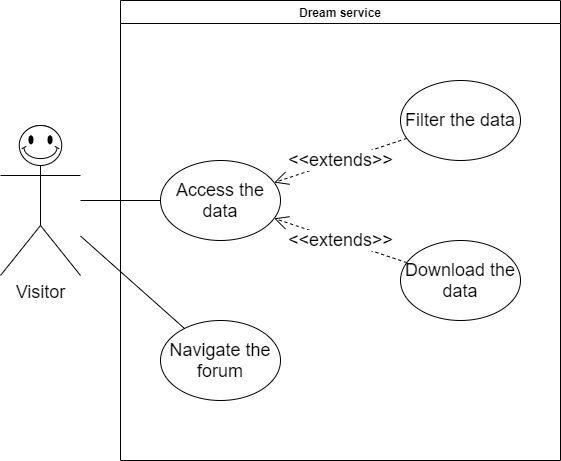
\includegraphics[scale=0.40]{images/use_cases_diagram/visitor_use_case.png}
        \caption{Use case diagram}
        \label{fig:vistor_use_case}
    \end{figure}
\FloatBarrier
    
\subsubsection*{Use case tables}

\begin{longtable}{p{.25\textwidth} | p{.75\textwidth}}
\caption{Filter data}
    \label{tab:filter_data}\\
        \hline
        \textbf{ID} & 1\\
        \hline
        \textbf{Name}  &  Filter data\\
        \hline
        \textbf{Actor}  &  Visitor\\
        \hline
        \textbf{Entry condition}  & The Visitor is in the Dream home page\\
    
        \hline
        \textbf{Events flow} & \begin{itemize}
                \item The Visitor clicks on the "Access the data" button
                \item The system displays the available data.
                \item The Visitor searches for the data set of interest
                \item The Visitor selects the “Filter” button on the data set he wants to filter
                \item The System pops up a list of different filters that can be applied to do a more precise search
                \item The Visitor select all the filters he wants to apply
                \item The Visitor clicks on the “Search” button
                \item The System search applying the selected filters

                \end{itemize}
                 \\
        \hline
        \textbf{Exit condition} & The new search is displayed\\
        \hline
    

    \end{longtable}
     \begin{figure}[h!]
        \centering
        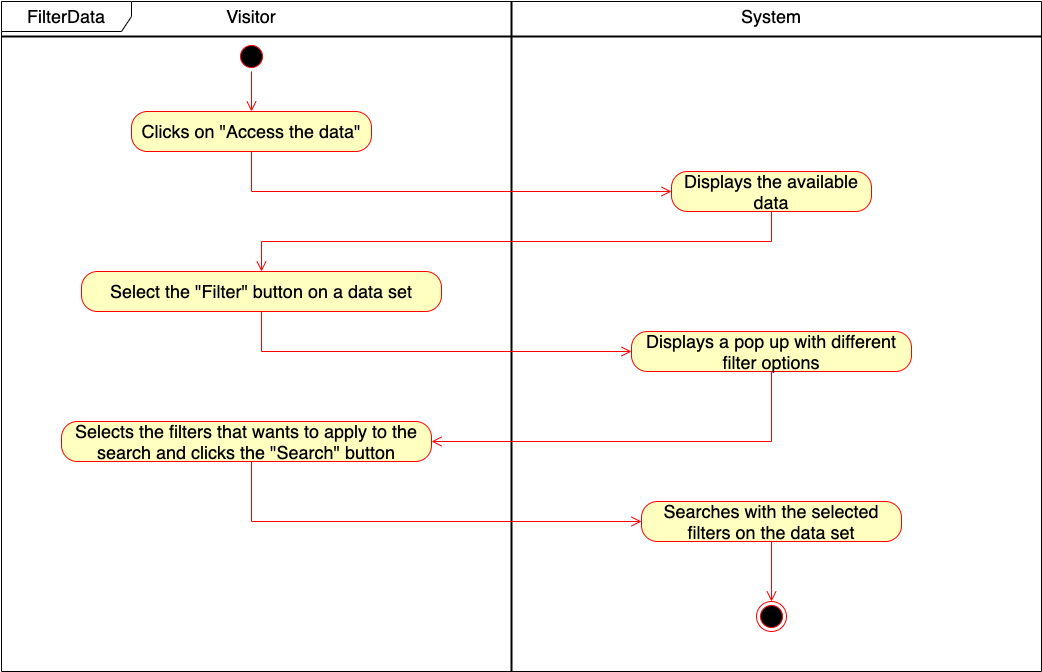
\includegraphics[scale=0.35]{images/use_cases_diagram/visitor_filter_data.png}
        \caption{Filter data}
        \label{fig:filter_data}
    \end{figure}
   
    \FloatBarrier
    \begin{longtable}{p{.25\textwidth} | p{.75\textwidth}}
    \caption{Download data set}
    \label{tab:download_dataset}\\
        \hline
        \textbf{ID} & 2\\
        \hline
        \textbf{Name}  &  Download data set\\
        \hline
        \textbf{Actor}  &  Visitor\\
        \hline
        \textbf{Entry condition}  &  The Visitor is in the Dream home page\\
        \hline
        \textbf{Events flow} & \begin{itemize}
                \item The Visitor clicks on the "Access the data" button
                \item The system displays the available data.
                \item The Visitor search for the data set of interest
                \item The Visitor select the “Download” button on the data set he wants to download
                \item The System pops up a data panoramic showing the different formats in which the data can be downloaded
                \item The Visitor select the data format he prefers
                \item The Visitor clicks on the “Download” button
                \item The System starts the download

                \end{itemize}
                 \\
        \hline
        \textbf{Exit condition} &  The data set is downloaded\\
        \hline
        \textbf{Output} & Data set\\
        \hline
    
    \end{longtable}
    \newpage
\begin{figure}[h!]
        \centering
        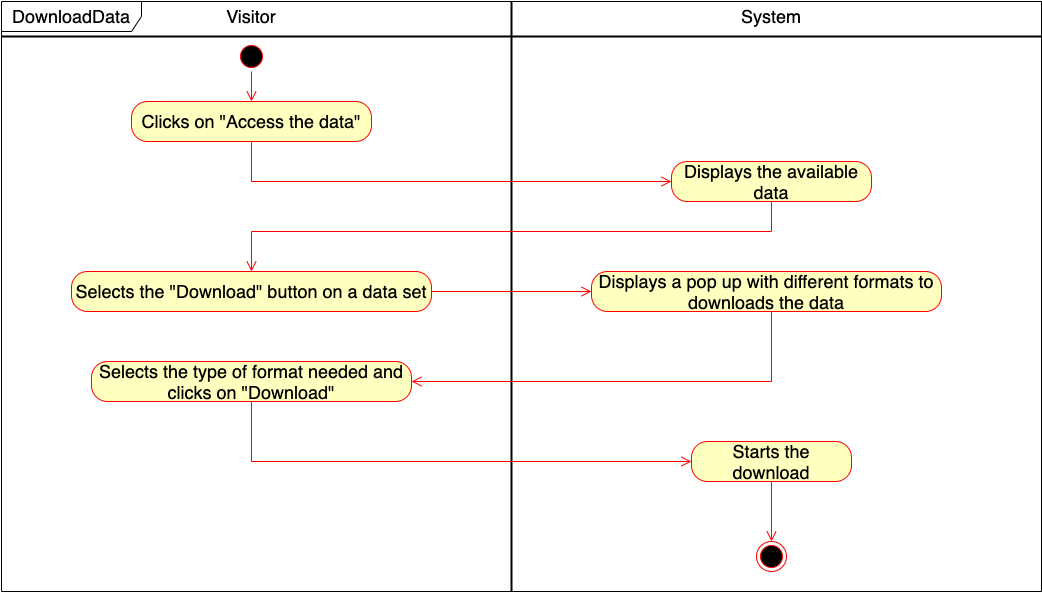
\includegraphics[scale=0.30]{images/use_cases_diagram/visitor_download_dataset.png}
        \caption{Download data set}
        \label{fig:download_data}
    \end{figure}
    \FloatBarrier
    
\begin{longtable}{p{.25\textwidth} | p{.75\textwidth}}
    \caption{Navigate the forum and download a document}
    \label{tab:navigate_forum}\\
        \hline
        \textbf{ID} & 3\\
        \hline
        \textbf{Name}  &  Navigate the forum and download a document\\
        \hline
        \textbf{Actor}  &  Visitor\\
        \hline
        \textbf{Entry condition}  &  The Visitor is in the Dream home page\\
        \hline
        \textbf{Events flow} & \begin{itemize}
                \item The Visitor click on "Open the forum" button
                \item The Visitor is redirected in the forum home page where all the topics are visible
                \item The Visitor click on the topic of his interest
                \item The System displays all the discussion related to the chosen topic
                \item The Visitor select the discussion he is interested in
                \item The system displays the discussion published by the Policy maker with all the replies from different users.
                \item The Visitor click and start the download of the attachment contained in the Policy maker's relation. 
                \end{itemize}
                 \\
        \hline
        \textbf{Exit condition} &  The visitor download the document\\
        \hline
        \textbf{Output} & Attachment \\ \hline
    
    \end{longtable}
\begin{figure}[h!]
        \centering
        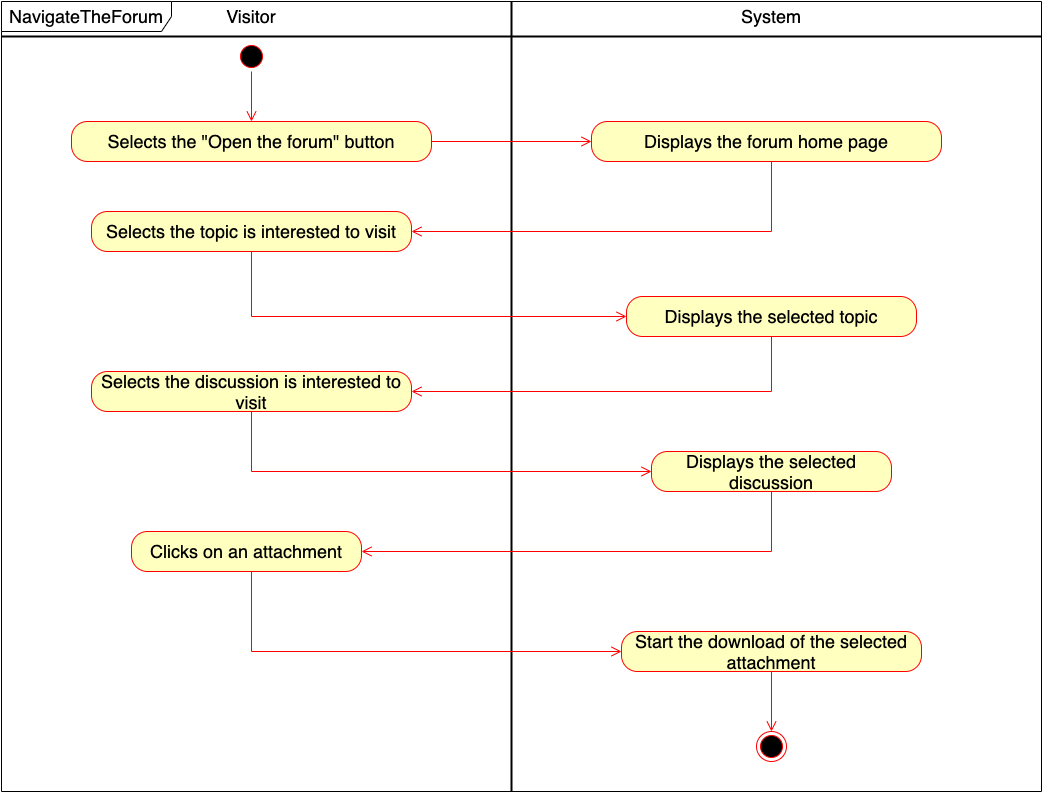
\includegraphics[scale=0.35]{images/use_cases_diagram/visitor_navigate_forum.png}
        \caption{Navigates the forum and download a document}
        \label{fig:navigate_forum}
    \end{figure}
    \FloatBarrier

\subsubsection{User scenarios}
\subsubsection*{Scenario 3}
Jishnu, a Telengana’s farmer, finds out about Dream forum and wants to read some posts. He clicks on the link found using a browser and selects his region, finding out the last review document published by a Policy maker. Once he has read the discussion he decides to make his contribution and shares the agricultural techniques he uses.
Jishnu hasn’t got an account yet, but he needs to be registered to post on the forum. For this purpose, he clicks on the “Sign up” button on the top right and he inserts his data in the following page, including the region in which he lives, his personal email address and eventually he chooses a safe password to protect his new account. Once he clicks on the confirmation button, the system tells him to check the email he has used to register to conclude the registration process. He opens his mail looking for a mail from Dream containing a confirmation link. When he clicks on it a browser page pops up containing a check message which confirms that the registration ended correctly. Now he can login from the home page, go to the page he was visiting and add his comment.

\subsubsection*{Scenario 4}
Basant is an active User of the forum of the site Dream. Unluckily, he discovers that the last post he published on a discussion contains a file that is not the file he wants to publish. So he returns to that post, clicks on the modify button and replaces the file with the correct one. After doing this procedure he clicks the confirmation button and then the changes to his post go to the pending approval list of the system.

\subsubsection*{Use case diagram}
\begin{figure}[h!]
        \centering
        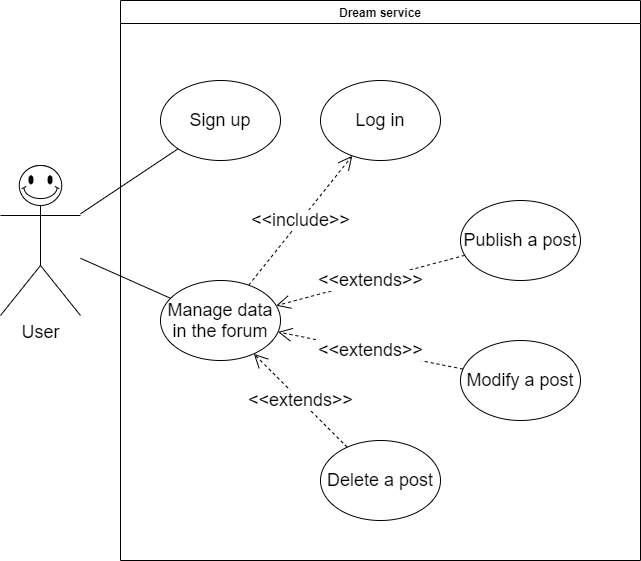
\includegraphics[scale=0.40]{images/use_cases_diagram/user_use_case.png}
        \caption{Use case diagram}
        \label{fig:user_use_case}
    \end{figure}
    
    \newpage
    
\subsubsection*{Use case tables}

\begin{longtable}{p{.25\textwidth} | p{.75\textwidth}}
 \caption{Sign Up User}
    \label{tab:sign_up}\\
        \hline
        \textbf{ID} & 4\\
        \hline
        \textbf{Name}  &  Sign up User\\
        \hline
        \textbf{Actor}  &  User\\
        \hline
        \textbf{Entry condition}  &  User has reached the site\\
        \hline
        \textbf{Input} & Personal data,
        email and password to use for the registration\\
        \hline
        \textbf{Events flow} & \begin{itemize}
                \item The site displays the “Sign up” button on the top right of the screen
                \item User clicks on “Sign up”
                \item The site displays a new page containing blank fields where user has to insert his data: name, surname, date of birth, area of residence, email and password
                \item User inserts the mandatory data and accepts the “Terms of Service”
                \item User confirms by clicking the confirmation button
                \item The page shows a message inviting User to visit his email address in order to conclude the registration
                \item User opens his inbox, find the email from Dream and clicks on confirmation link
                \item The site displays a confirmation message of successful registration
                \end{itemize}
                 \\
        \hline
        \textbf{Exit condition} & User registration has been successful: the inserted data are stored in the database of the system. Now User can login using his credentials and post in the forum\\
        \hline
        \textbf{Output} & Registration data are stored in the database of Dream site.\\
        \hline
        \textbf{Exception} & \begin{itemize}
            \item User inserts non valid data(e.g. wrong email format or nonexistent area). The application displays an error message telling the User that he must check the data inserted and correct the invalid ones
            \item User inserts an e-mail which is already stored in the in the database. So, after user inserts his data and clicks on confirm, the application displays an error message telling User that he’s already registered to the service and invites him to login with that email
    \end{itemize} \\\hline
   
    \end{longtable}
     
     \begin{figure}[h!]
        \centering
        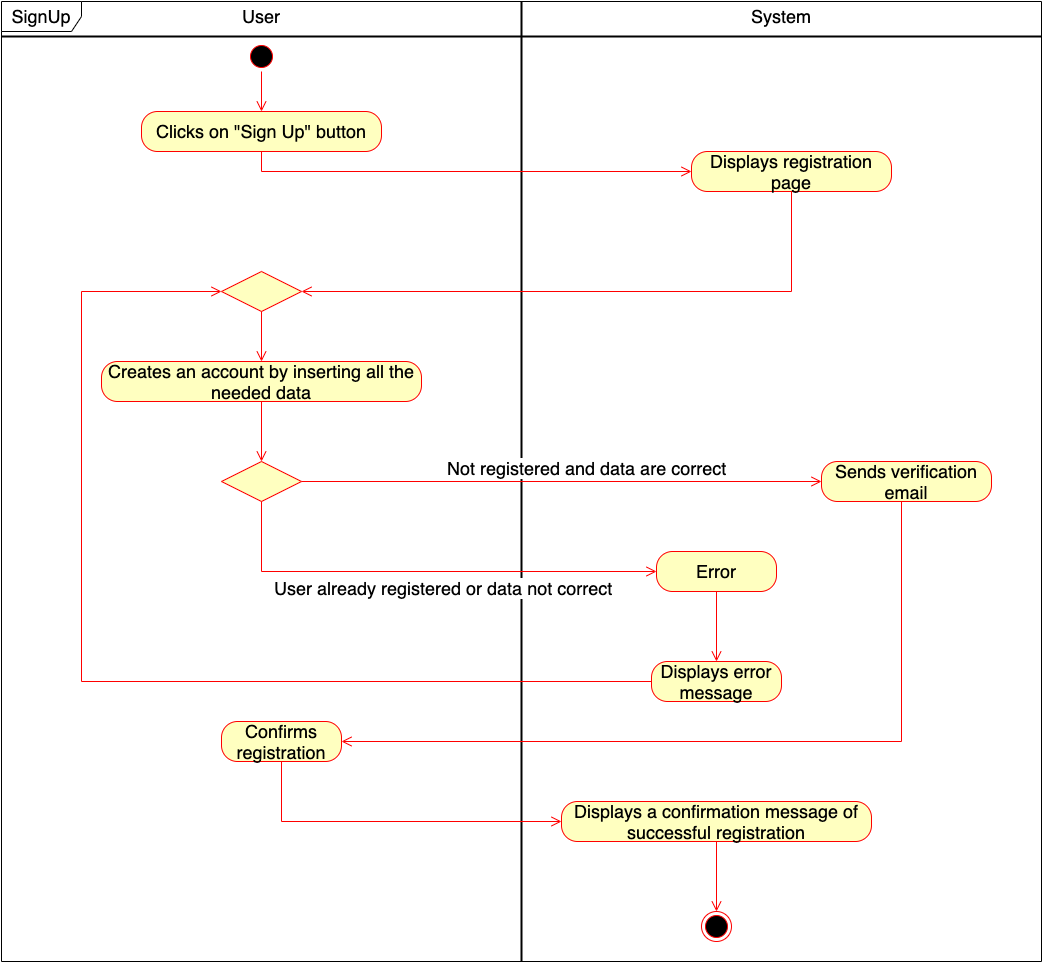
\includegraphics[scale=0.35]{images/use_cases_diagram/user_sign_up.png}
        \caption{Sign Up  User}
        \label{fig:usr_sign_up}
    \end{figure}
     \FloatBarrier
     
    \begin{longtable}{p{.25\textwidth} | p{.75\textwidth}}
     \caption{Login User}
        \label{tab:login_user}\\
        \hline
        \textbf{ID} & 5\\
        \hline
        \textbf{Name}  &  Login User\\
        \hline
        \textbf{Actor}  &  User\\
        \hline
        \textbf{Entry condition}  &  
        \begin{itemize}
                \item User has reached the site
                \item User is already registered to the platform
         \end{itemize}\\
        \hline
        \textbf{Input} & User email and password associated to a successful registration\\
        \hline
        \textbf{Events flow} & 
        \begin{itemize}
                \item The site displays the “Sign In” button on the top right of the screen
                \item User clicks on “Sign In”
                \item The system displays the login page
                \item User fills the username (email) and password fields using the credential inserted during the registration
                \item System checks the validity of the credentials inserted
                \item The system displays the precedent page or, if unavailable, the home page of the site
                 \end{itemize}
                 \\
        \hline
        \textbf{Exit condition} & User is logged in\\
        \hline
        \textbf{Exceptions} & User inserts wrong credentials and clicks on “login” button. The system shows an error message inviting the User to check the credentials before trying again to login\\
        \hline
       
    \end{longtable}
    \begin{figure}[h!]
        \centering
        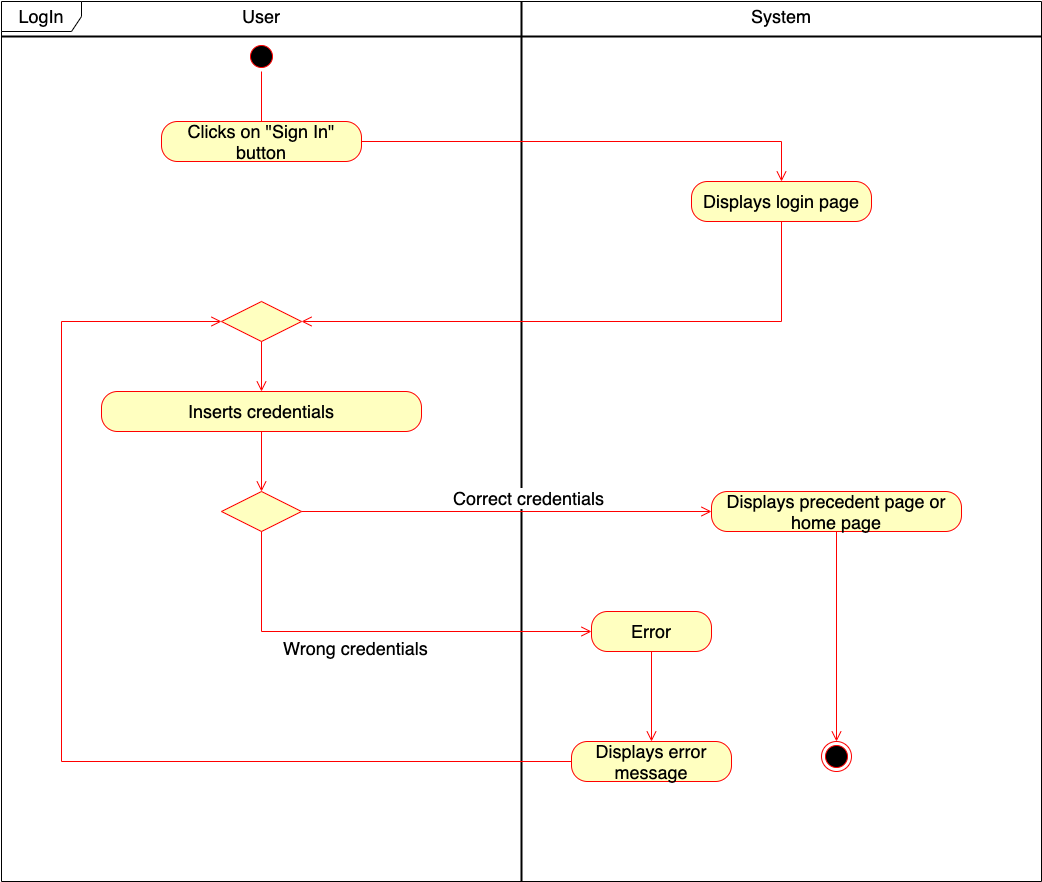
\includegraphics[scale=0.35]{images/use_cases_diagram/user_login.png}
        \caption{Login User}
        \label{fig:user_login}
    \end{figure}
    \FloatBarrier
    
    \begin{longtable}{p{.25\textwidth} | p{.75\textwidth}}
    \caption{Publish a post by User}
        \label{tab:publish_post_by_user}\\
        \hline
        \textbf{ID} & 6\\
        \hline
        \textbf{Name}  &  Publish a post by User\\
        \hline
        \textbf{Actor}  &  User\\
        \hline
        \textbf{Entry condition}  &  
        \begin{itemize}
                \item The User is already registered in the system
                \item The User is already logged in the system
                \item The User is in the forum home page
         \end{itemize}\\
        \hline
        \textbf{Input} & Post\\
        \hline
        \textbf{Events flow} & 
        \begin{itemize}
                \item The User selects the section of his interest
                \item The User selects the discussion about the argument of interest
                \item The User inserts a new answer in the form
                \item The User confirms the answer by clicking the confirmation button
                 \end{itemize}
                 \\
        \hline
        \textbf{Exit condition} & The answer is in pending approval\\
        \hline
        \textbf{Exceptions} & The User tries to insert invalid contents (invalid characters, invalid file format, etc...)\\
        \hline
        
    \end{longtable}
    
    \begin{figure}[h!]
        \centering
        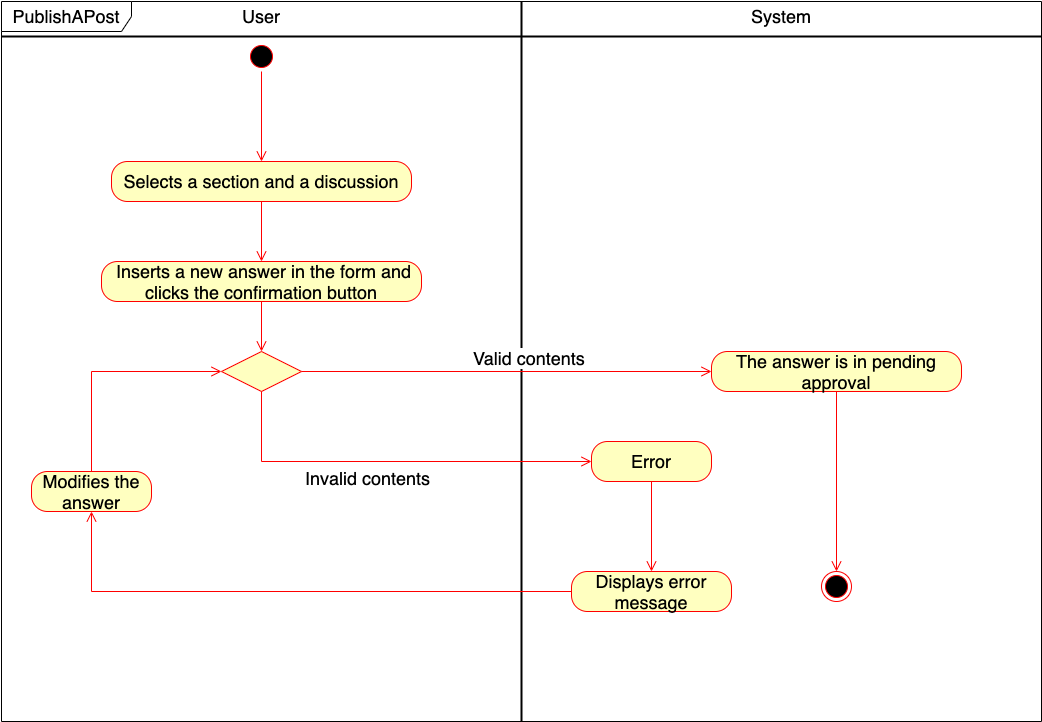
\includegraphics[scale=0.35]{images/use_cases_diagram/user_publish_post.png}
        \caption{Publish a post by User}
        \label{fig:publish_post_by_user}
    \end{figure}
   \newpage
    \begin{longtable}{p{.25\textwidth} | p{.75\textwidth}}
    \caption{Modify a post by User}
        \label{tab:modify_post_by_user}\\
        \hline
        \textbf{ID} & 7\\
        \hline
        \textbf{Name}  &  Modify a post by User\\
        \hline
        \textbf{Actor}  &  User\\
        \hline
        \textbf{Entry condition}  &  
        \begin{itemize}
                \item The User is already registered in the system
                \item The User is already logged in the system
                \item The User is in the discussion page where the post is present
                \item The User has already published the post
         \end{itemize}\\
        \hline
        \textbf{Input} & Post\\
        \hline
        \textbf{Events flow} & 
        \begin{itemize}
                \item The User press on the “Modify” button on the selected post
                \item The System returns to the User the edit page
                \item The User introduces the changes in the post
                \item The User confirms the changes by clicking the confirmation button

                 \end{itemize}
                 \\
        \hline
        \textbf{Exit condition} & The changes to the post are visible\\
        \hline
        \textbf{Exceptions} &  The User  tries to insert invalid contents (invalid characters, invalid file format, etc...)\\
        \hline
        \textbf{Special requirements} & The User can modify only post written by his account \\ \hline
        
    \end{longtable}
    \begin{figure}[h!]
        \centering
        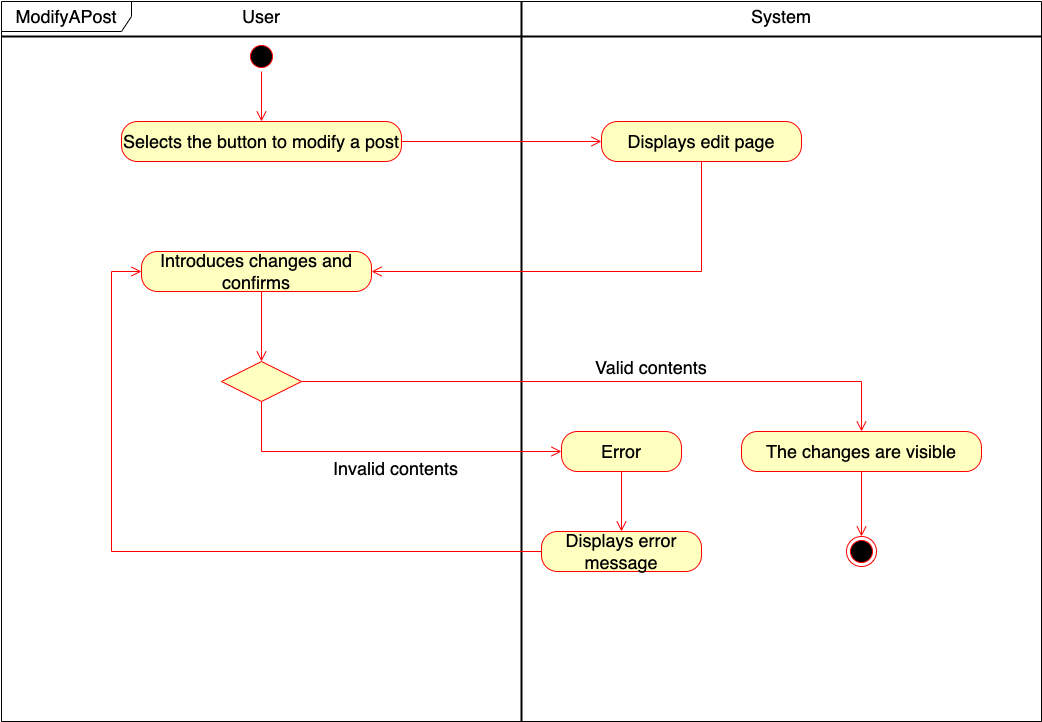
\includegraphics[scale=0.35]{images/use_cases_diagram/user_modify_post.png}
        \caption{Modify a post by User}
        \label{fig:user_modify_post}
    \end{figure}
    \FloatBarrier
    
                \begin{longtable}{p{.25\textwidth} | p{.75\textwidth}}
        \caption{Delete a post by User}
    \label{tab:user_delete_post}\\
        \hline
        \textbf{ID} & 8\\
        \hline
        \textbf{Name}  &  Delete post by User\\
        \hline
        \textbf{Actor}  &  User\\
        \hline
        \textbf{Entry condition}  &  \begin{itemize}
            \item  The User is already registered in the system
            \item  The User is already logged in the system
            \item  The User is in the discussion page where the post is present
            \item The User has already published the post
        \end{itemize}\\
        \hline
        \textbf{Input} & Post\\
        \hline
        \textbf{Events flow} & \begin{itemize}
                \item The User press on the “Delete” button on the selected post
                \item The System returns to the User a confirmation message
                \item The User confirms the operation by clicking the confirmation button
                \end{itemize}
                 \\
        \hline
        \textbf{Exit condition} & The post is deleted from the forum\\
        \hline
        \textbf{Exception} & The User doesn't confirm the operation\\ \hline
        \textbf{Special requirements} & The User can delete only post written by his account \\ \hline

    
    \end{longtable}
      \begin{figure}[h!]
        \centering
        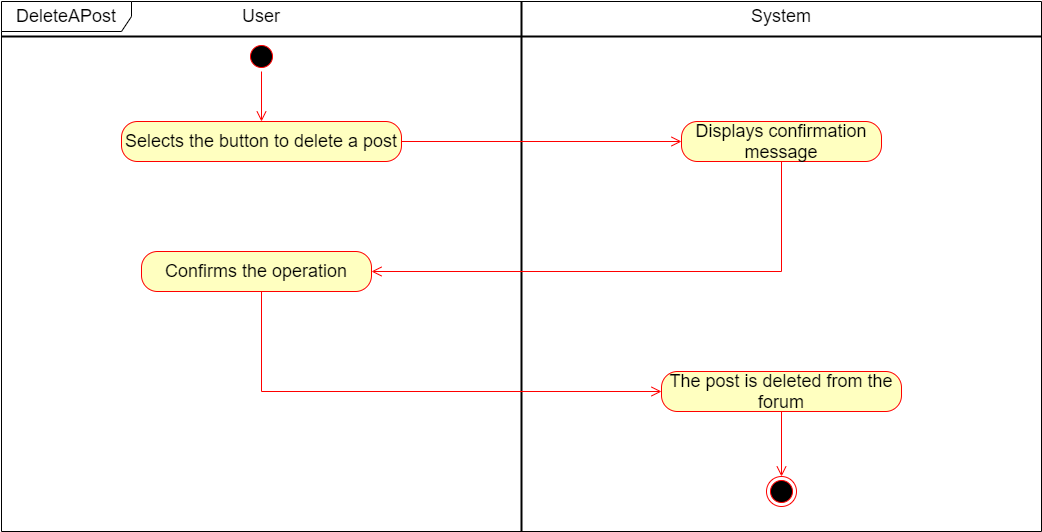
\includegraphics[scale=0.35]{images/use_cases_diagram/user_delete_post.png}
        \caption{Delete a post by User}
        \label{fig:user_delete_post}
    \end{figure}
    \FloatBarrier
    
\subsubsection{Policy maker scenarios}
\subsubsection*{Scenario 5}
Gurleen, a Telengana’s Policy maker, needs to visualize data about agricultural harvest quality. Gurleen connects at Dream’s site and lands at the home page. She clicks a button in the top right of the screen with the words “Sign In”. Gurleen is already registered to the service, so she authenticates digiting her email and password and accesses to her reserved area. From this screen she accesses the Deviance section and from that point she can visualize a ranking list, established by Dream project’s service, of the different areas. At this point, she identifies the areas with the best score and publishes a document, publicly visible, where she asks to the farmers to present a report about their cultivation techniques, that will be published in the forum.

\subsubsection*{Scenario 6}
Digamber, another Policy maker from the same area of Gurleen, checks his email and notice a notification from Dream about a new publication in a discussion that he has created. Clicking on the link from the email he opens the correspondent forum discussion. Once he has read Gurleeen’s replies he notice that he can’t answer because he isn’t logged in. So he clicks the “Sign In” button in the top right and he fills the fields with his username and password to authenticate. In this way he can write his replies and publish it in the discussion.

\subsubsection*{Scenario 7}
Bipin is a Telengana’s Policy maker. His boss asked him to check the efficiency of agricultural production in the district of Medak. Bipin goes to the Dream site home page and since is the first time he’s assigned this job he has firstly to register to the portal. He clicks on the “Registration” button on the top right and inserts his data in the following page. He’s asked for his personal code (Policy maker ID) which identifies him as Policy maker and eventually he confirms data insertion. A mail is send to the email address used during the registration with a confirmation link that once clicked consent to activate the new account. Bipin clicks on it and land on a confirmation page.

\subsubsection*{Scenario 8}
Akash is a Policy maker of Telengana and needs to manage the forum of the Dream’s site. Akash then connects to the home page of the Dream’s site and since he is already logged in, he can go directly on the forum page, by clicking a button present on the home page. When he reaches the forum, Akash clicks on the “Moderator area”, then he selects the pending list option and from that moment he can see a pending list with all the posts that required approval before being published in the forum. Akash decides to open the first post, examine it and then he approves it to be published; after the confirmation by Akash, the system automatically publishes the post in the forum and sends a notification to the author of the post.

\subsubsection*{Scenario 9}
Parag is a Policy maker already registered in Dream’s site. Today he needs to recalculate the Deviance according to certain parameters, told by his boss. So since he is already logged in, he can go directly to his reserved area, by clicking a button present on the home page. After doing that he selects the Deviance section and from that moment he can see the actual ranking list, calculated by default by the system, and a list of parameters that he can select in order to recalculate a custom Deviance. He selects on three different parameters and then clicks on recalculate. The system recalculates the Deviance and then reloads the contents, showing the new custom ranking list.

\subsubsection*{Use case diagram}
\begin{figure}[h!]
        \centering
        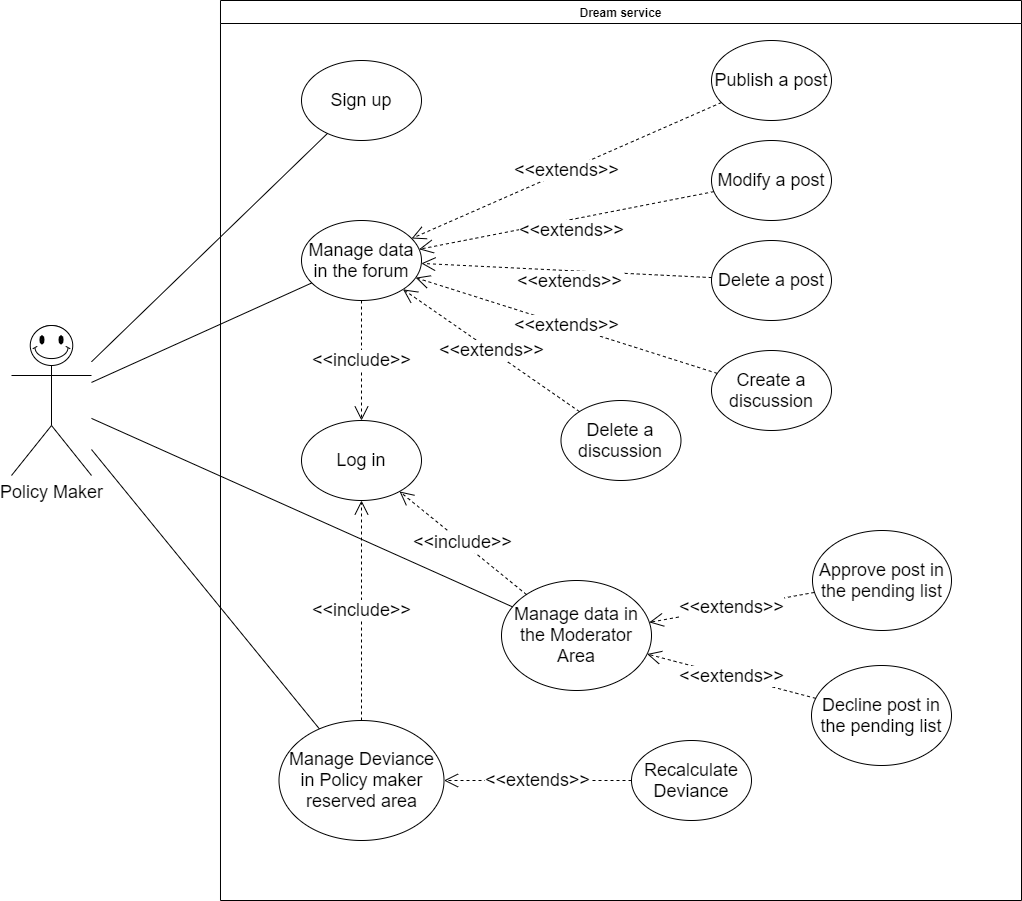
\includegraphics[scale=0.35]{images/use_cases_diagram/policymaker_use_case.png}
        \caption{Use case diagram}
        \label{fig:policy_maker_use_case}
    \end{figure}
 \newpage
\subsubsection*{Use case tables}

\begin{longtable}{p{.25\textwidth} | p{.75\textwidth}}
\caption{Sign Up Policy maker}
        \label{tab:signup_policy_maker}\\
        \hline
        \textbf{ID} & 9\\
        \hline
        \textbf{Name}  &  Sign up Policy maker\\
        \hline
        \textbf{Actor}  &  Policy maker\\
        \hline
        \textbf{Entry condition}  &  Policy maker has reached the site\\
        \hline
        \textbf{Input}  & Personal data, Policy maker ID, email and password to use for the registration\\ 
        \hline
        \textbf{Events flow} & 
        \begin{itemize}
                \item The site displays the “Sign Up” button on the top right of the screen
                \item Policy maker clicks on “Sign Up”
                \item The site displays a new page containing blank fields where user has to insert his data: name, surname, Policy maker ID, date of birth, area of residence, email and password
                \item Policy maker inserts the mandatory data and the Policy maker ID
                \item Policy maker confirms by clicking the confirmation button
                \item The page shows a message inviting Policy maker to visit his email address in order to conclude the registration
                \item Policy maker opens his inbox, find the email from Dream and clicks on confirmation link
                \item The site displays a confirmation message of successful registration
                 \end{itemize}
                 \\
        \hline
        \textbf{Exit condition} & Policy maker registration has been successful: the inserted data are stored in the database of the system. Now Policy maker can login using his credentials and post in the forum\\
        \hline
        \textbf{Output} & Registration data are stored in the database of Dream site.\\
        \hline
        \textbf{Exceptions} & 
        \begin{itemize}
            \item Policy maker inserts non valid data (wrong date format or nonexistent area). The application displays an error message telling the Policy maker that he must check the data inserted and correct the invalid ones. 
            \item Policy maker inserts an email which is already stored in the database. So, after user inserts his data and clicks on confirm, the application displays an error message telling User that he’s already registered to the service and invites him to login with that email
            \item Policy maker inserts a non valid ID
            \item Policy maker inserts data non corresponding to the ID
        \end{itemize}\\
        \hline
       
        
    \end{longtable}

\begin{figure}[h!]
        \centering
        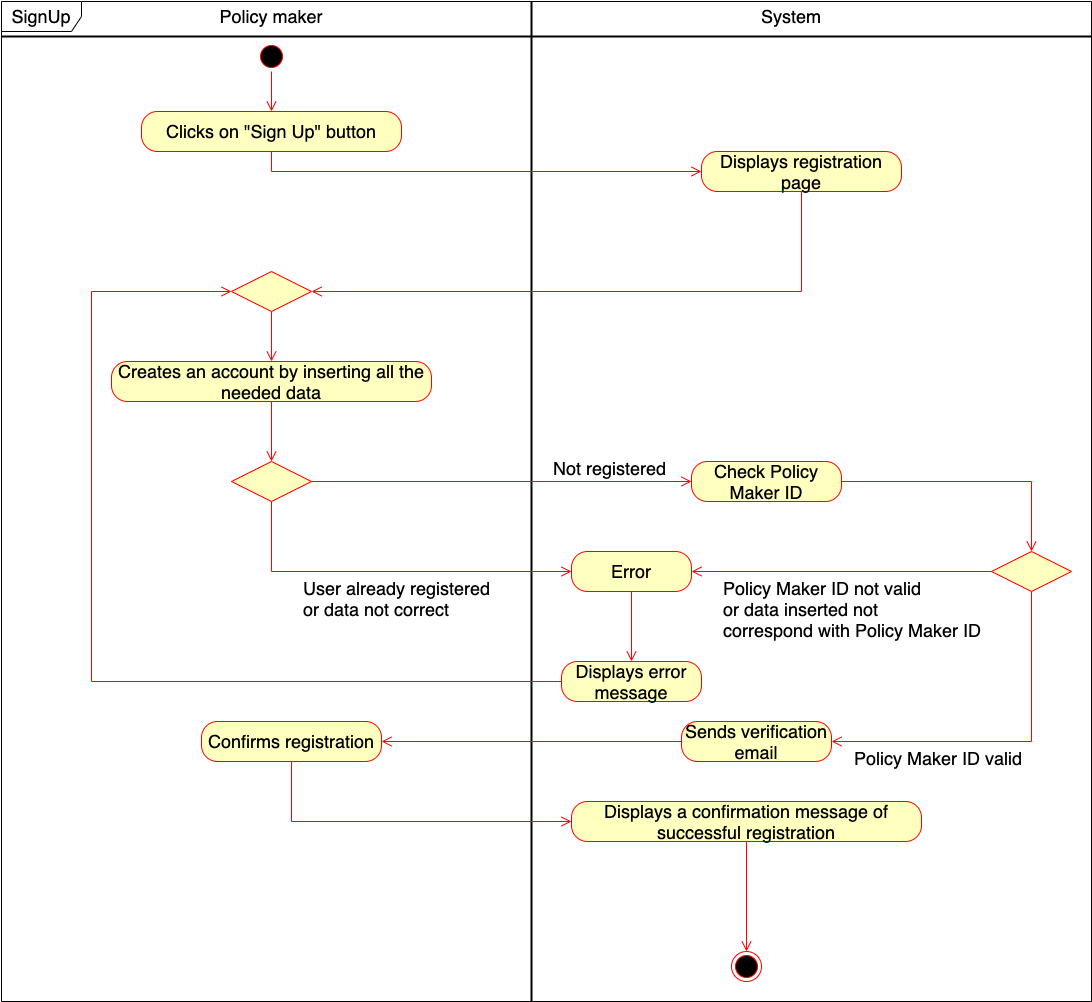
\includegraphics[scale=0.30]{images/use_cases_diagram/policymaker_sign_up.png}
        \caption{Sign Up Policy maker}
        \label{fig:policymaker_sign_up}
    \end{figure}
\FloatBarrier

\begin{longtable}{p{.25\textwidth} | p{.75\textwidth}}
\caption{Login Policy maker}
        \label{tab:login_policy_maker}\\
        \hline
        \textbf{ID} & 10\\
        \hline
        \textbf{Name}  &  Login Policy maker \\
        \hline
        \textbf{Actor}  &  Policy maker\\
        \hline
        \textbf{Entry condition}  &  
        \begin{itemize}
                \item Policy maker has reached the site
                \item Policy maker is already registered to the platform
         \end{itemize}\\
        \hline
        \textbf{Input}  & Policy maker email and password associated to a successful registration\\ 
        \hline
        \textbf{Events flow} & 
        \begin{itemize}
                \item The site displays the “Sign in” button on the top right of the screen
                \item Policy maker clicks on “Sign In"
                \item The system displays the login page
                \item Policy maker fills the username (email) and password fields using the credential inserted during the registration
                \item System checks the validity of the credentials inserted
                \item The system displays the precedent page or, if unavailable, the home page of the Policy maker dashboard
                 \end{itemize}
                 \\
        \hline
        \textbf{Exit condition} & Policy maker is logged in\\
        \hline
        \textbf{Exceptions} & Policy maker inserts wrong credentials and clicks on login button. The system shows an error message inviting the Policy maker to check the credentials before trying again to login\\
        \hline
       
        
    \end{longtable}
    
    \begin{figure}[h!]
        \centering
        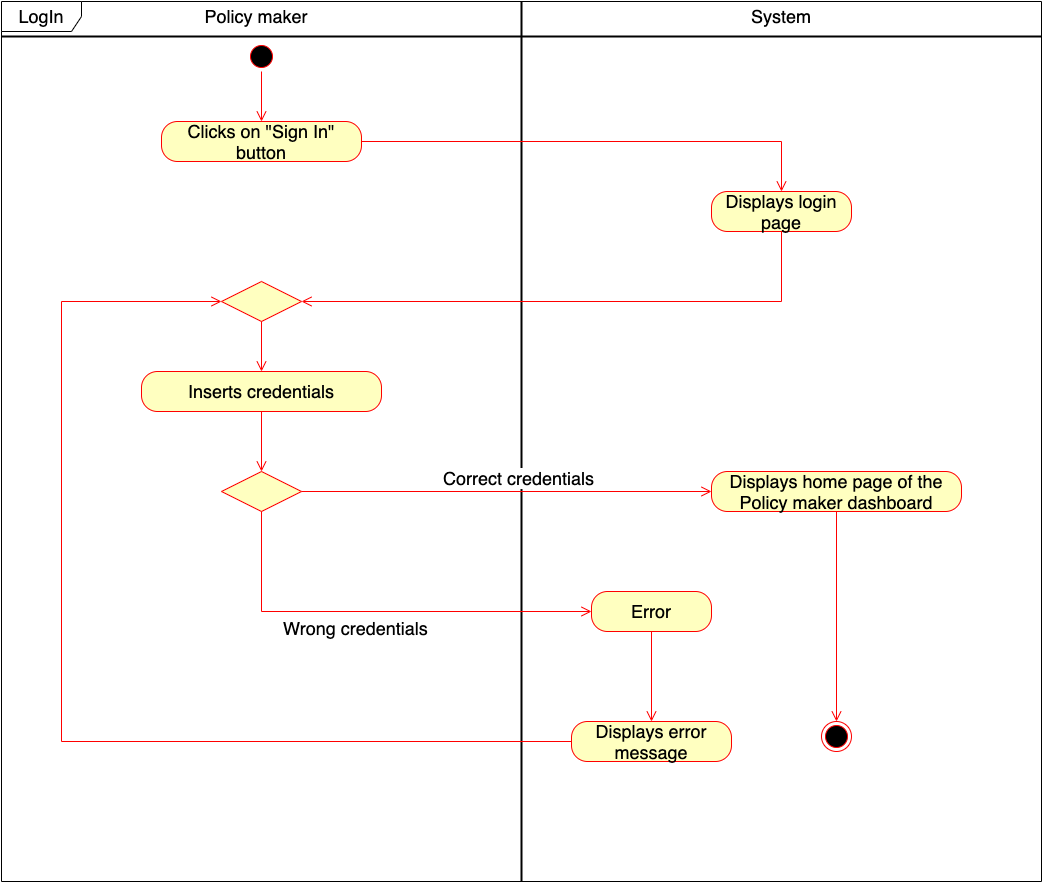
\includegraphics[scale=0.35]{images/use_cases_diagram/policymaker_login.png}
        \caption{Login Policy maker}
        \label{fig:policymaker_login}
    \end{figure}
    \FloatBarrier
    
    \begin{longtable}{p{.25\textwidth} | p{.75\textwidth}}
    \caption{Publish a post by Policy maker}
        \label{tab:publish_post_by_policy_maker}\\
        \hline
        \textbf{ID} & 11\\
        \hline
        \textbf{Name}  &  Publish a post by Policy maker\\
        \hline
        \textbf{Actor}  &  Policy maker\\
        \hline
        \textbf{Input}  &  Post\\
        \hline
        \textbf{Entry condition}  &  
        \begin{itemize}
                \item The Policy maker is already registered in the system
                \item The Policy maker is already logged in the system
                \item The Policy maker is in the forum home page
         \end{itemize}\\
        \hline
        \textbf{Events flow} & 
        \begin{itemize}
                \item The Policy maker selects the section of his interest
                \item The Policy maker selects the discussion about the argument of interest
                \item The Policy maker inserts a new answer in the form
                \item The Policy maker confirms the answer by clicking the confirmation button
                 \end{itemize}
                 \\
        \hline
        \textbf{Exit condition} & The answer is published\\
        \hline
        \textbf{Exceptions} & The Policy maker tries to insert non valid contents (invalid characters, invalid file format, etc...)\\
        \hline
       
    \end{longtable}
    
    \begin{figure}[h!]
        \centering
        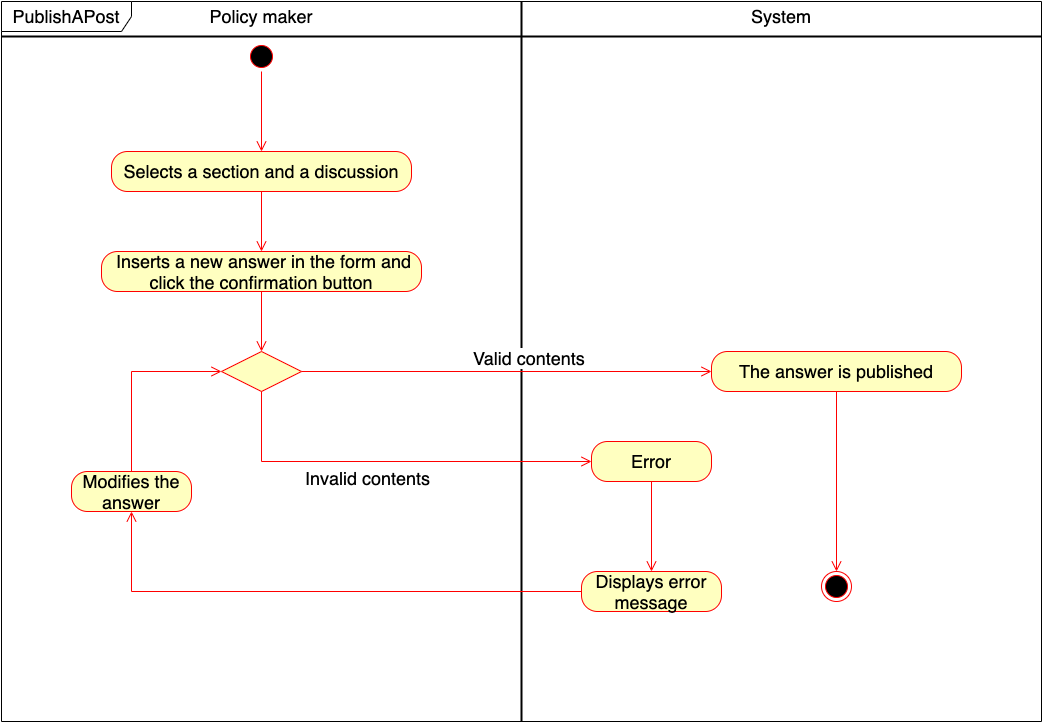
\includegraphics[scale=0.35]{images/use_cases_diagram/policymaker_publish_post.png}
        \caption{Publish a post by Policy maker}
        \label{fig:policymaker_publish_post}
    \end{figure}
\FloatBarrier

\newpage

    \begin{longtable}{p{.25\textwidth} | p{.75\textwidth}}
        \caption{Modify a post by Policy maker}
    \label{tab:pm_modify_post}\\
        \hline
        \textbf{ID} & 12\\
        \hline
        \textbf{Name}  &  Modify a post by Policy maker\\
        \hline
        \textbf{Actor}  &  Policy maker\\
        \hline
        \textbf{Entry condition}  &  \begin{itemize}
            \item  The Policy maker is already registered in the system
            \item  The Policy maker is already logged in the system
            \item  The Policy maker is in the discussion page where the post is present
        \end{itemize}\\
        \hline
        \textbf{Input} & Post\\
        \hline
        \textbf{Events flow} & \begin{itemize}
                \item The Policy maker press on the “Modify” button on the selected post
                \item The System returns to the Policy maker the edit page
                \item The Policy maker introduces the changes in the post
                \item The Policy maker confirms the changes by clicking the confirmation button
                \end{itemize}
                 \\
        \hline
        \textbf{Exit condition} & The changes are introduced in the post\\
        \hline
        \textbf{Exception} & The Policy maker tries to insert invalid contents (invalid characters, invalid file format, etc...)\\ \hline
        \textbf{Special requirements} & The Policy maker can modify every post \\ \hline
    \end{longtable}
    \begin{figure}[h!]
        \centering
        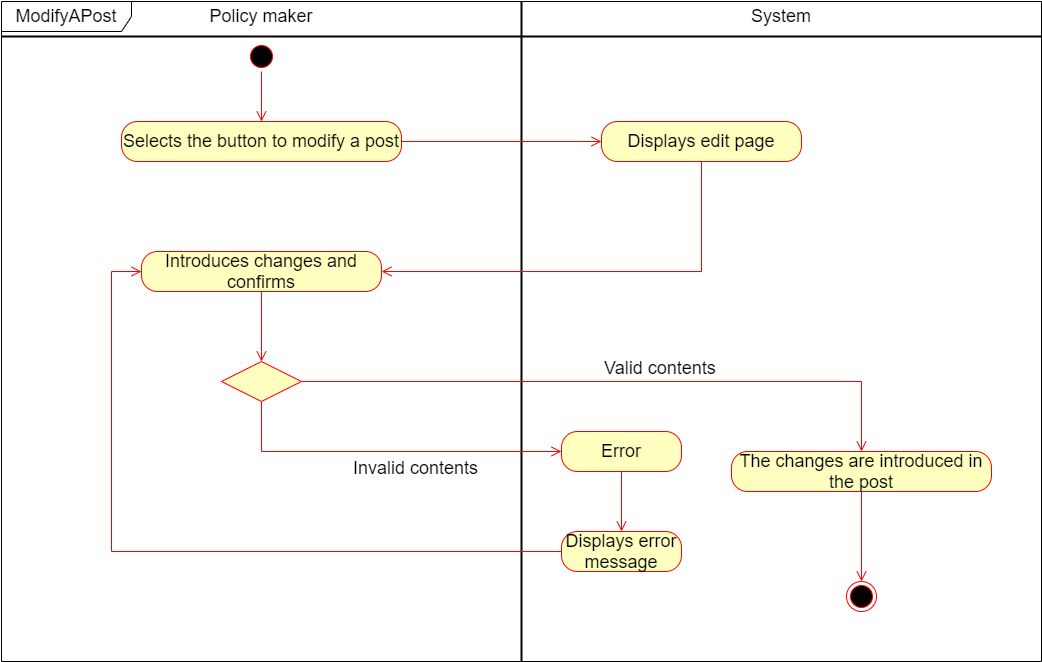
\includegraphics[scale=0.35]{images/use_cases_diagram/policymaker_modify_post.png}
        \caption{Modify a post by Policy maker}
        \label{fig:policymaker_modify_post}
    \end{figure}
    \FloatBarrier

\begin{longtable}{p{.25\textwidth} | p{.75\textwidth}}
        \caption{Delete a post by Policy maker}
    \label{tab:pm_delete_post}\\
        \hline
        \textbf{ID} & 13\\
        \hline
        \textbf{Name}  &  Delete a post by Policy maker\\
        \hline
        \textbf{Actor}  &  Policy maker\\
        \hline
        \textbf{Entry condition}  &  \begin{itemize}
            \item  The Policy maker is already registered in the system
            \item  The Policy maker is already logged in the system
            \item The post is already published
            \item  The Policy maker is in the discussion page where the post is present
        \end{itemize}\\
        \hline
        \textbf{Input} & Post\\
        \hline
        \textbf{Events flow} & \begin{itemize}
                \item The Policy maker press on the “Delete” button on the selected post
                \item The System returns to the Policy maker a confirmation message
                \item The Policy maker confirms the operation by clicking the confirmation button
                \end{itemize}
                 \\
        \hline
        \textbf{Exit condition} & The post is deleted from the forum\\
        \hline
        \textbf{Exception} & The Policy maker doesn't confirm the operation\\ \hline
        \textbf{Special requirements} & The Policy maker can delete every post\\ \hline

    \end{longtable}
    
    \begin{figure}[h!]
        \centering
        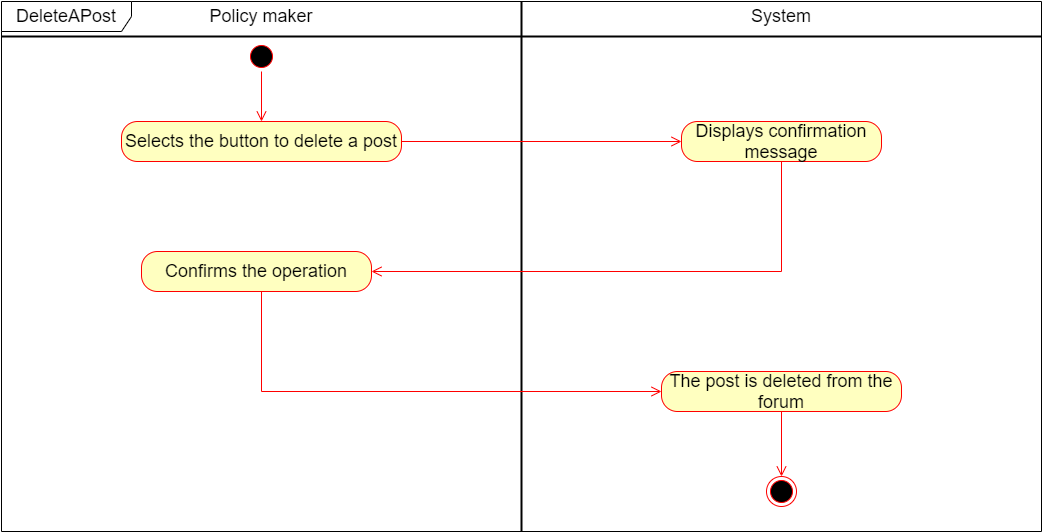
\includegraphics[scale=0.38]{images/use_cases_diagram/policymaker_delete_post.png}
        \caption{Delete a post by Policy maker}
        \label{fig:policymaker_delete_post}
    \end{figure}
    \FloatBarrier
    \newpage
    \begin{longtable}{p{.25\textwidth} | p{.75\textwidth}}
    \caption{Create a new discussion}
    \label{tab:create_new_discussion}\\
        \hline
        \textbf{ID} & 14\\
        \hline
        \textbf{Name}  &  Create a new discussion\\
        \hline
        \textbf{Actor}  &  Policy maker\\
        \hline
        \textbf{Entry condition}  &  \begin{itemize}
            \item The Policy maker is already registered in the system
            \item The Policy maker is already logged in the system
            \item The Policy maker is in the forum home page
        \end{itemize}\\
        \hline
        \textbf{Events flow} & \begin{itemize}
                \item The Policy maker selects the topic of his interest
                \item The Policy maker click on the “New discussion” button
                \item The Policy maker writes/uploads the report 
                \item The Policy maker confirms the operation by clicking on the confirmation button
                \end{itemize}
                 \\
        \hline
        \textbf{Exit condition} & The report is saved and published in the system\\
        \hline
        \textbf{Exception} & The Policy maker tries to insert invalid contents\\\hline
    
    \end{longtable}
    
    \begin{figure}[h!]
        \centering
        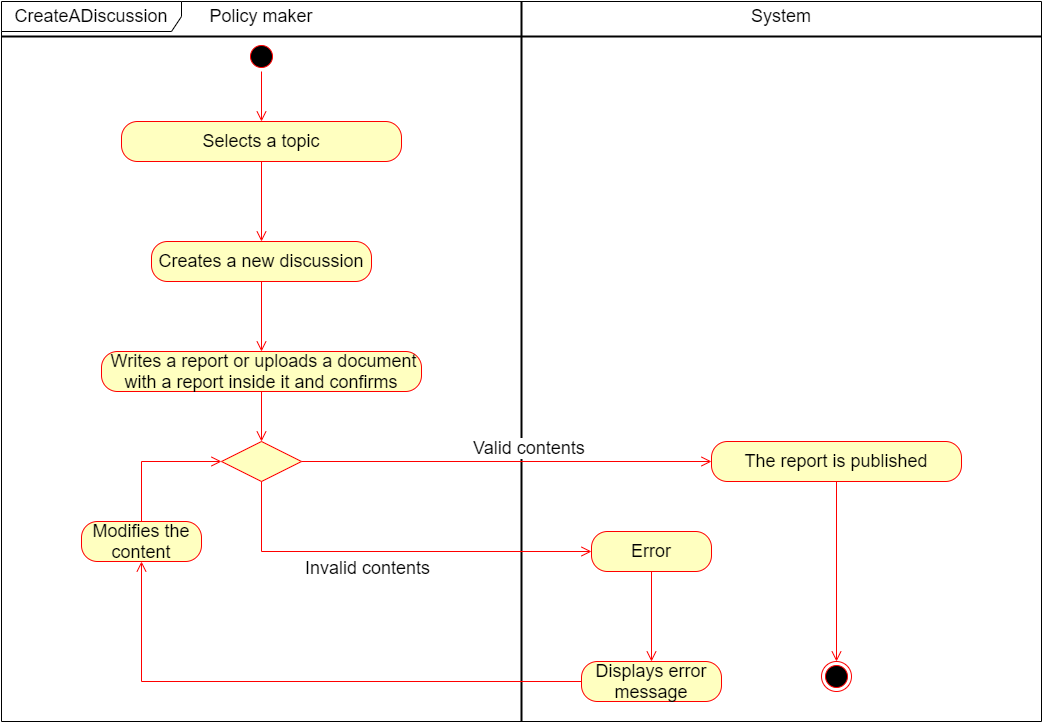
\includegraphics[scale=0.35]{images/use_cases_diagram/policymaker_create_discussion.png}
        \caption{Create a new discussion}
        \label{fig:policymaker_create_discussion}
    \end{figure}
 \FloatBarrier
 
 \begin{longtable}{p{.25\textwidth} | p{.75\textwidth}}
        \caption{Delete a discussion}
    \label{tab:pm_delete_discussion}\\
        \hline
        \textbf{ID} & 15\\
        \hline
        \textbf{Name}  &  Delete a discussion\\
        \hline
        \textbf{Actor}  &  Policy maker\\
        \hline
        \textbf{Entry condition}  &  \begin{itemize}
            \item  The Policy maker is already registered in the system
            \item  The Policy maker is already logged in the system
            \item The discussion is already existing
            \item  The Policy maker is in the topic where the discussion is present
        \end{itemize}\\
        \hline
        \textbf{Input} & Discussion\\
        \hline
        \textbf{Events flow} & \begin{itemize}
                \item The Policy maker press on the “Delete” button on the selected discussion
                \item The System returns to the Policy maker a confirmation message
                \item The Policy maker confirms the operation by clicking the confirmation button
                \end{itemize}
                 \\
        \hline
        \textbf{Exit condition} & The discussion and all the posts inside of it are deleted from the forum\\
        \hline
        \textbf{Exception} & The Policy maker doesn't confirm the operation\\ \hline
        \textbf{Special requirements} & The Policy maker can delete every discussion\\ \hline

    \end{longtable}
    
    \begin{figure}[h!]
        \centering
        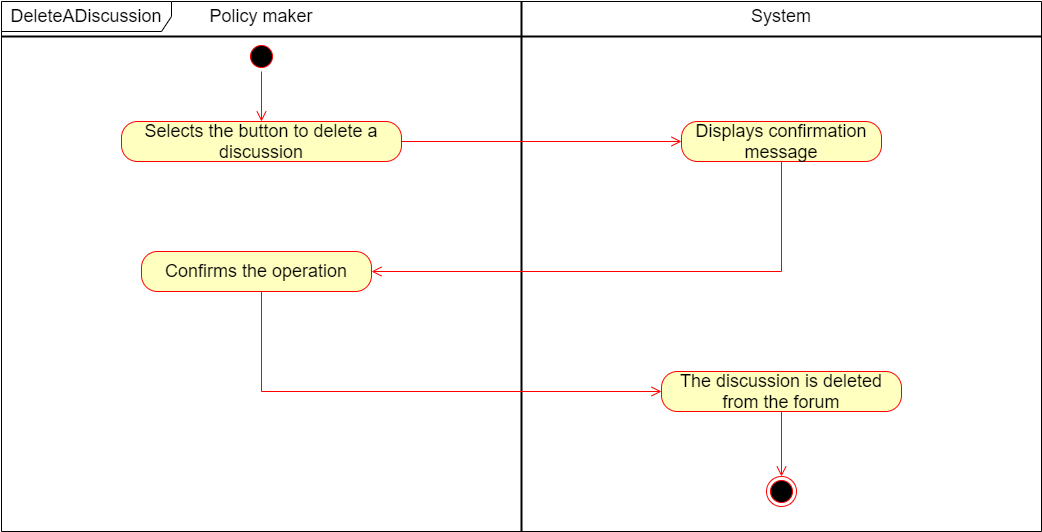
\includegraphics[scale=0.38]{images/use_cases_diagram/policymaker_delete_discussion.png}
        \caption{Delete a discussion}
        \label{fig:policymaker_delete_discussion}
    \end{figure}
    \FloatBarrier
    \newpage
    \begin{longtable}{p{.25\textwidth} | p{.75\textwidth}}
     \caption{Confirm pending post}
        \label{tab:Confirm_pending_post}\\
        \hline
        \textbf{ID} & 16\\
        \hline
        \textbf{Name}  &  Confirm pending post\\
        \hline
        \textbf{Actor}  &  Policy maker\\
        \hline
        \textbf{Entry condition}  &  
        \begin{itemize}
                \item The Policy maker is already registered in the system
                \item The Policy maker is already logged in the system
                \item The Policy maker is in the forum home page
         \end{itemize}\\
        \hline
        \textbf{Events flow} & 
        \begin{itemize}
                \item The Policy maker selects the “Moderator Area” button
                \item The system displays the Moderator Area
                \item The Policy maker selects the “pending list” option
                \item The system displays the pending post list
                \item The Policy maker selects a pending post request
                \item The system displays the selected post
                \item The Policy maker reviews the post
                \item The Policy maker approves the post by clicking on the confirmation button
                 \end{itemize}
                 \\
        \hline
        \textbf{Exit condition} &
        \begin{itemize}
                \item The post is removed from the pending list and published in the forum
                \item A notification is sent to the Author of the post
                \end{itemize}
                \\
        \hline
        \textbf{Special Requirements} & The pending post must be accepted no later than 30 days after it is sent by User\\
        \hline
       
       
    \end{longtable}
    

    \begin{longtable}{p{.25\textwidth} | p{.75\textwidth}}
     \caption{Decline pending post}
    \label{tab:decline_pending_post}\\
        \hline
        \textbf{ID} & 17\\
        \hline
        \textbf{Name}  &  Decline pending post\\
        \hline
        \textbf{Actor}  &  Policy maker\\
        \hline
        \textbf{Entry condition}  &  \begin{itemize}
            \item The Policy maker is already registered in the system
            \item The Policy maker is already logged in the system
            \item The Policy maker is in the forum home page

        \end{itemize}\\
        \hline
        \textbf{Events flow} & \begin{itemize}
                \item The Policy maker selects the “Moderator Area” button
                \item The system displays the Moderator Area
                \item The Policy maker selects the “pending list” option 
                \item The system displays the pending post list
                \item The Policy maker selects a pending post request
                \item The Policy maker reviews the post
                \item The Policy maker declines the approval of the post by clicking on the decline button
                \end{itemize}
                 \\
        \hline
        \textbf{Exit condition} & \begin{itemize}
            \item The pending post request is deleted and removed from the pending post list
            \item A notification is sent to the Author of the post
        \end{itemize}\\
        \hline
   
    \end{longtable}
\begin{figure}[h!]
        \centering
        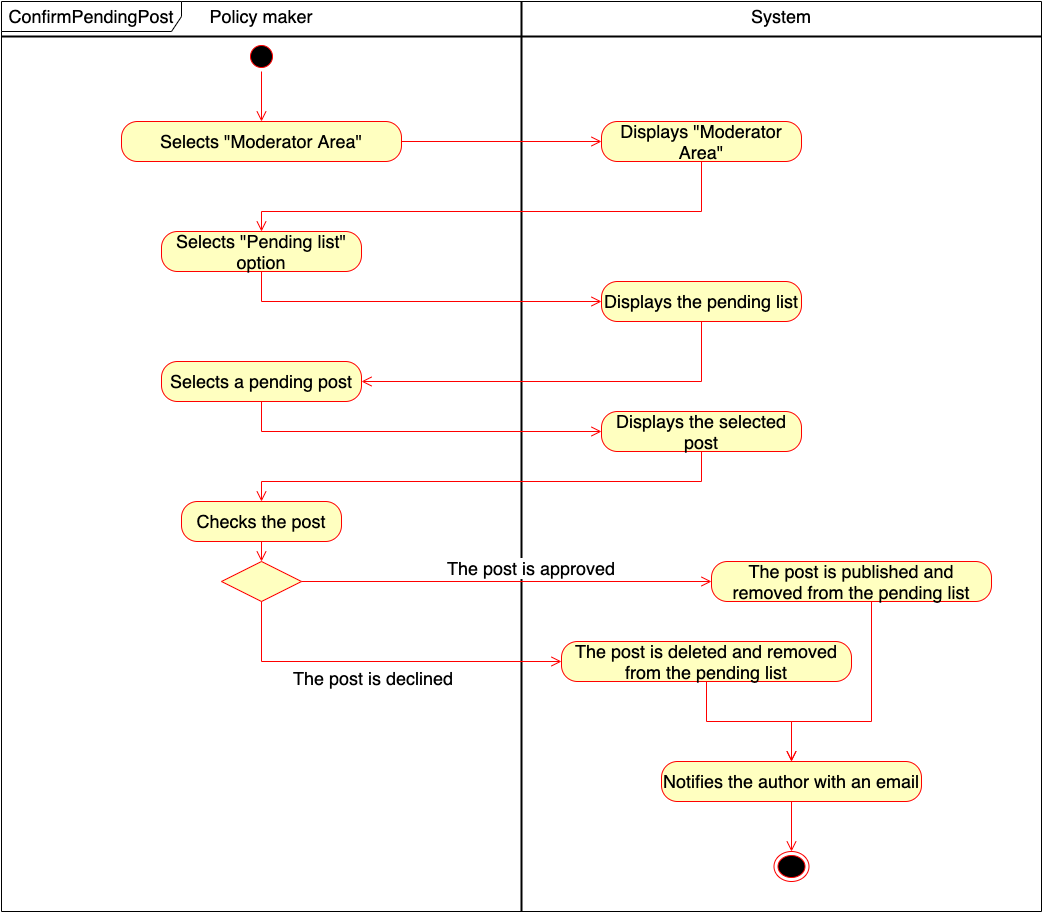
\includegraphics[scale=0.35]{images/use_cases_diagram/policymaker_pending_post.png}
        \caption{Confirm or decline a pending post}
        \label{fig:policymaker_pending_post}
    \end{figure}
\FloatBarrier
    
    \newpage
    
          \begin{longtable}{p{.25\textwidth} | p{.75\textwidth}}
          \caption{Recalculate new deviance}
    \label{tab:recalculate_new_deviance}\\
        \hline
        \textbf{ID} & 18\\
        \hline
        \textbf{Name}  &  Recalculate new Deviance\\
        \hline
        \textbf{Actor}  &  Policy maker\\
        \hline
        \textbf{Entry condition}  &  \begin{itemize}
            \item The Policy maker is already registered in the system
            \item The Policy maker is already logged in the system
            \item The Policy maker is in the home page
        \end{itemize}\\
        \hline
        \textbf{Input} & Parameters and data\\
        \hline
        \textbf{Events flow} & \begin{itemize}
                \item The Policy maker selects the “Reserved Area” button
                \item The System displays the Reserved Area
                \item The Policy maker selects the “Deviance” option
                \item The System displays the actual Deviance, calculated by default by the system, and a list of parameters that he can select in order to recalculate a custom Deviance
                \item The Policy maker selects different parameters
                \item The Policy maker clicks on Recalculate
                \item The System recalculate the new Deviance
                \item The System displays the new ranking list

                \end{itemize}
                 \\
        \hline
        \textbf{Exit condition} & The Deviance is recalculated and it's displayed the new ranking list\\
        \hline
        \textbf{Exception} & The Policy maker didn’t selects any parameter\\ \hline
        
    
    \end{longtable}
    
    \begin{figure}[h!]
        \centering
        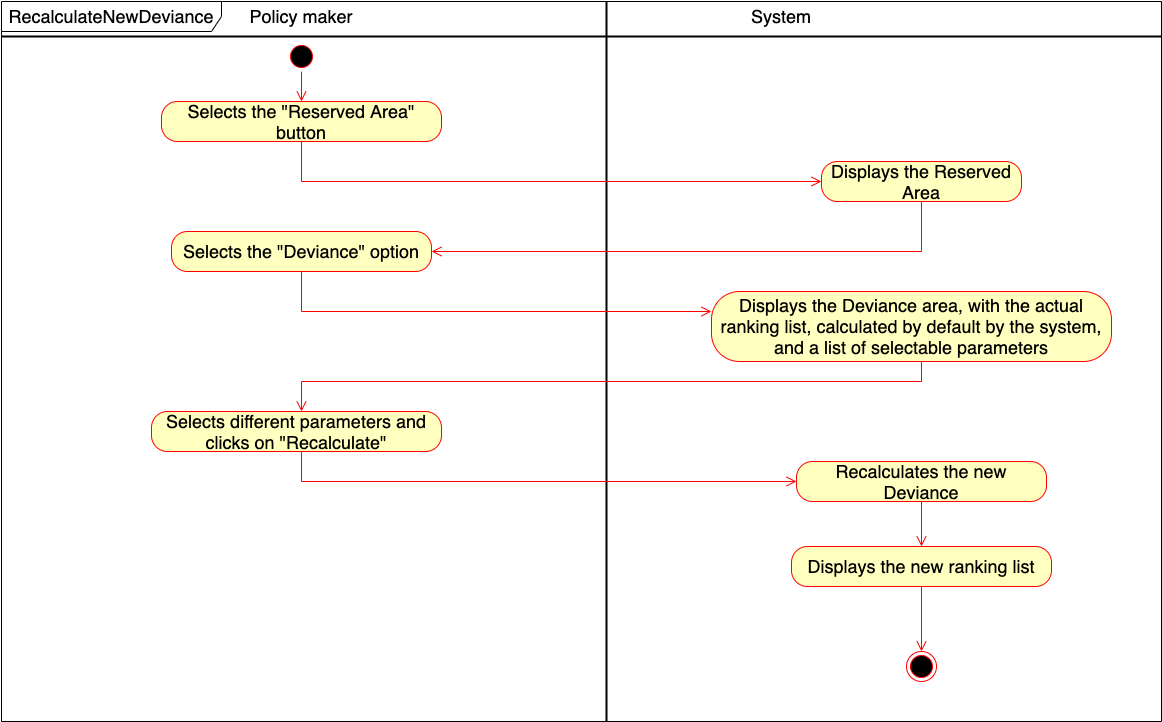
\includegraphics[scale=0.35]{images/use_cases_diagram/policymaker_recalculate_deviance.png}
        \caption{Recalculate new deviance}
        \label{fig:policymaker_recalculate_deviance}
    \end{figure}
    \FloatBarrier



\subsubsection{Administrator scenarios}
\subsubsection*{Scenario 10}
Alessandro is an administrator of the Dream system and wants to add a new data source. He connects to the administration site and login using his administrator credentials. On the administration screen he selects the “Manage data sources” section. He clicks on the button to add a new data source and inserts the source link from where the data will be recovered and clicks on the import button.
\newpage
\subsubsection*{Use case diagram}
\begin{figure}[h!]
        \centering
        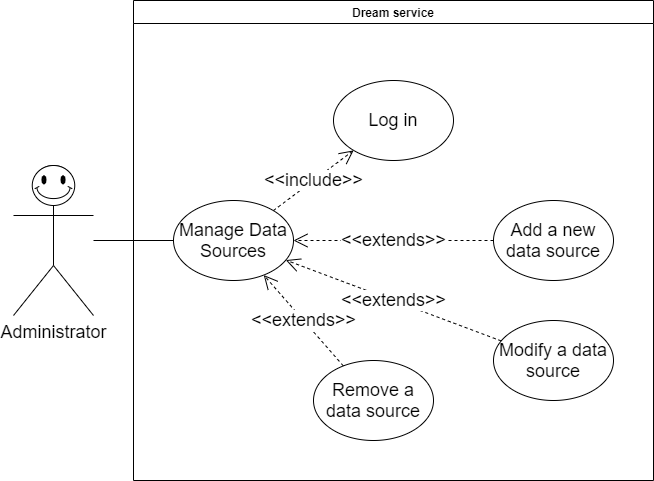
\includegraphics[scale=0.40]{images/use_cases_diagram/administrator_use_case.png}
        \caption{Use case diagram}
        \label{fig:administrator_use_case}
    \end{figure}
    \FloatBarrier
\subsubsection*{Use case tables}
\begin{longtable}{p{.25\textwidth} | p{.75\textwidth}}
\caption{Login Administrator}
        \label{tab:login_administrator}\\
        \hline
        \textbf{ID} & 19\\
        \hline
        \textbf{Name}  &  Login Administrator \\
        \hline
        \textbf{Actor}  &  Administrator\\
        \hline
        \textbf{Entry condition}  &  
        \begin{itemize}
                \item Administrator has reached the administration site
         \end{itemize}\\
        \hline
        \textbf{Input}  & Administrator's email and password\\ 
        \hline
        \textbf{Events flow} & 
        \begin{itemize}
            
                \item The system displays the login page
                \item Administrator fills the username (email) and password fields using the credential
                \item System checks the validity of the credentials inserted
                \item The system displays the precedent page or, if unavailable, the home page of the administration dashboard
                 \end{itemize}
                 \\
        \hline
        \textbf{Exit condition} & Administrator is logged in\\
        \hline
        \textbf{Exceptions} & Administrator inserts wrong credentials and clicks on “login” button. The system shows an error message inviting the Administrator to check the credentials before trying again to login\\
        \hline
       
        
    \end{longtable}
    
    \begin{figure}[h!]
        \centering
        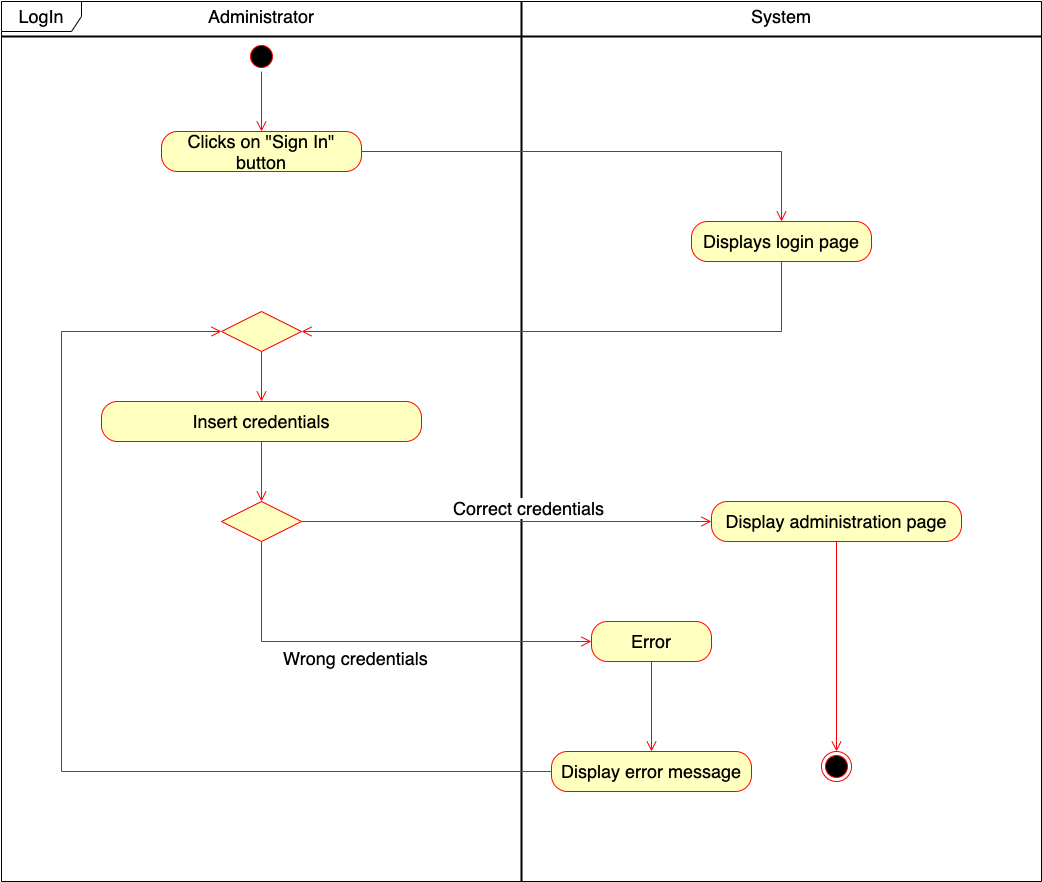
\includegraphics[scale=0.35]{images/use_cases_diagram/administrator_login.png}
        \caption{Login Administrator}
        \label{fig:administrator_login}
    \end{figure}
 \FloatBarrier   
 
 \newpage
 
\begin{longtable}{p{.25\textwidth} | p{.75\textwidth}}
    \caption{Add new data source}
        \label{tab:add_new_data_source}\\
        \hline
        \textbf{ID} & 20\\
        \hline
        \textbf{Name}  &  Add new data source \\
        \hline
        \textbf{Actor}  &  Administrator\\
        \hline
        \textbf{Input}  &  Data source to add\\
        \hline
        \textbf{Entry condition}  &  
        \begin{itemize}
                \item The Administrator is already registered in the system
                \item The Administrator is already logged in the system
                \item The Administrator is in the admin home page
         \end{itemize}\\
        \hline
        \textbf{Events flow} & 
        \begin{itemize}
                \item The Administrator selects the “Data sources” section
                \item The System opens the “Data sources” page
                \item The Administrator clicks on the button to add a new source
                \item The System render the form to add a new source
                \item The Administrator compile the form with the new data source’s origin
                \item The Administrator confirms the operation 
                 \end{itemize}
                 \\
        \hline
        \textbf{Exit condition} & The new data source is available on the site\\
        \hline
        \textbf{Exceptions} & 
        \begin{itemize}
                \item The Administrator tries to insert an unavailable source
                \item The Administrator tries to insert a data source already present in the system
                \end{itemize}
                \\
        \hline
        \textbf{Special requirements}  &  The Administrator needs to have the copyright permission to use the data source\\
        \hline
       
        
    \end{longtable}
    
    \begin{figure}[h!]
        \centering
        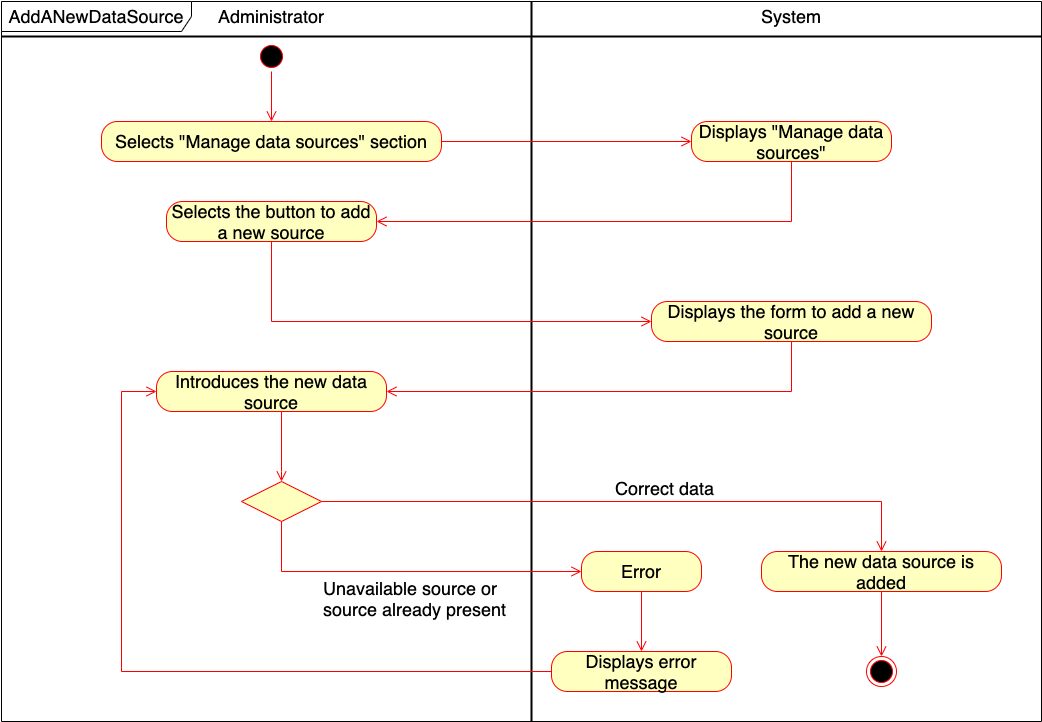
\includegraphics[scale=0.35]{images/use_cases_diagram/administrator_add_datasource.png}
        \caption{Add new data source}
        \label{fig:administrator_add_datasource}
    \end{figure}
   \FloatBarrier 
   
   \begin{longtable}{p{.25\textwidth} | p{.75\textwidth}}
     \caption{Modify a data source}
        \label{tab:modify_data_source}\\
        \hline
        \textbf{ID} & 21\\
        \hline
        \textbf{Name}  &  Modify a data source\\
        \hline
        \textbf{Actor}  &  Administrator\\
        \hline
        \textbf{Input}  &  Changes to a data source\\
        \hline
        \textbf{Entry condition}  &  
        \begin{itemize}
                \item The Administrator is already registered in the system
                \item The Administrator is already logged in the system
                \item The Administrator is in the admin home page
         \end{itemize}\\
        \hline
        \textbf{Events flow} & 
        \begin{itemize}
                \item The Administrator selects the “Data sources” section
                \item The System opens the “Data sources” page
                \item The Administrator clicks on the “Modify” button associated to the data source he wants to modify
                \item The System render a form, from which the administrator could modify some data 
                \item The Administrator modify some parameters of the selected data source
                \item The Administrator confirms the operation 
                 \end{itemize}
                 \\
        \hline
        \textbf{Exit condition} & The data source is modified and is available on the site\\
        \hline
        \textbf{Exceptions} &  
        \begin{itemize}
            \item The Administrator doesn’t confirm the operation
            \item The changes results in equivalence with another existing data source
        \end{itemize}\\
        \hline
        \textbf{Special requirements} &  The Administrator needs to have the copyright permission to use the data source\\
        \hline
       
        
    \end{longtable}

    \begin{figure}[h!]
        \centering
        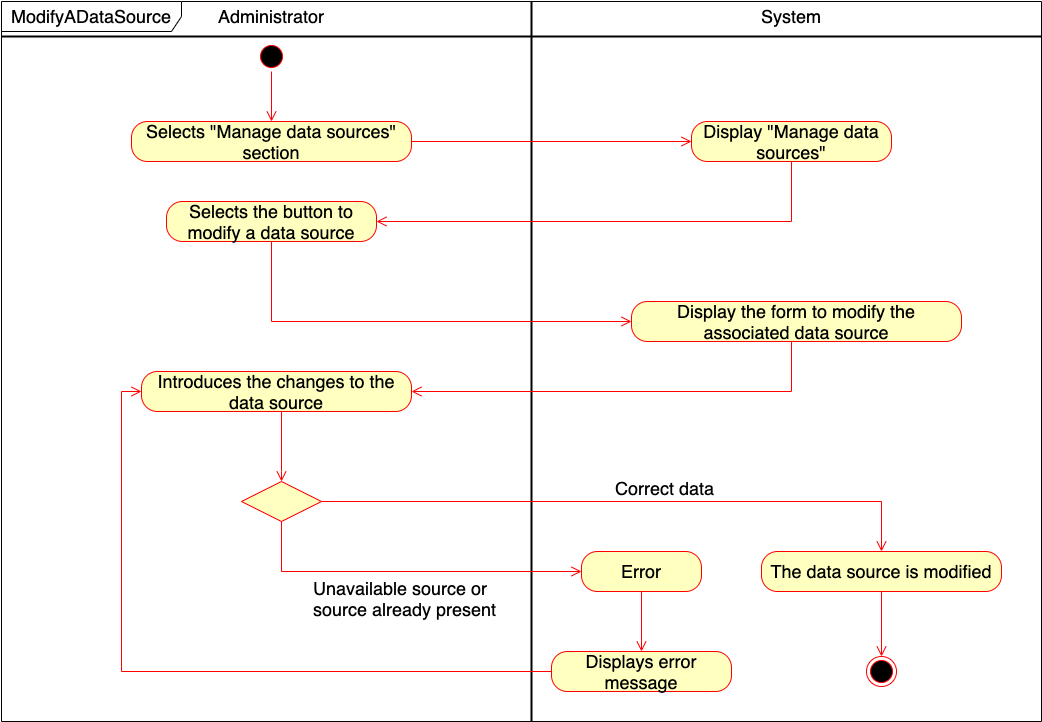
\includegraphics[scale=0.35]{images/use_cases_diagram/administrator_modify_datasource.png}
        \caption{Modify a data source}
        \label{fig:administrator_modify_datasource}
    \end{figure}
    \FloatBarrier
   
    \begin{longtable}{p{.25\textwidth} | p{.75\textwidth}}
     \caption{Remove a data source}
        \label{tab:remove_data_source}\\
        
        \hline
        \textbf{ID} & 22\\
        \hline
        \textbf{Name}  &  Remove a data source\\
        \hline
        \textbf{Actor}  &  Administrator\\
        \hline
        \textbf{Input}  &  Data source to remove\\
        \hline
        \textbf{Entry condition}  &  
        \begin{itemize}
                \item The Administrator is already registered in the system
                \item The Administrator is already logged in the system
                \item The Administrator is in the admin home page
         \end{itemize}\\
        \hline
        \textbf{Events flow} & 
        \begin{itemize}
                \item The Administrator selects the “Data sources” section
                \item The System opens the “Data sources” page
                \item The Administrator clicks on the button to remove a data source, associated to the data source he wants to remove
                \item The System render an alert asking for confirmation to remove the data source
                \item The Administrator confirms the operation 
                 \end{itemize}
                 \\
        \hline
        \textbf{Exit condition} & The data source is no more available in the system\\
        \hline
        \textbf{Exceptions} &  The Administrator doesn’t confirm the operation\\
        \hline
       
       
    \end{longtable}
    
    \begin{figure}[h!]
        \centering
        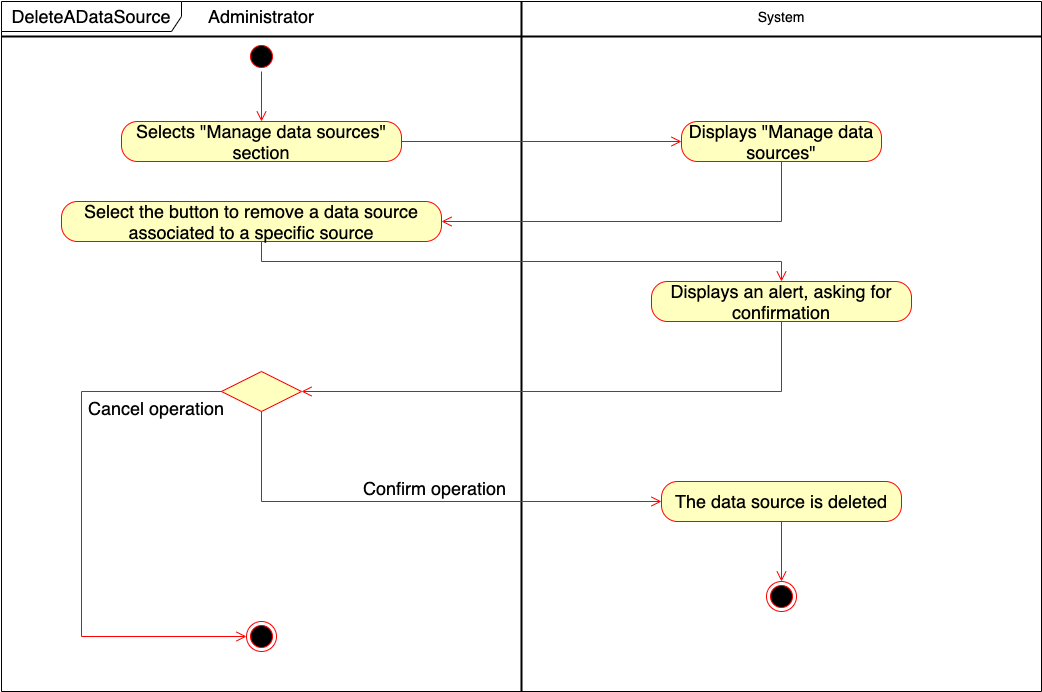
\includegraphics[scale=0.35]{images/use_cases_diagram/administrator_delete_datasource.png}
        \caption{Remove a data source}
        \label{fig:administrator_remove_datasource}
    \end{figure}
 \FloatBarrier   
 
 \newpage

\subsubsection{Requirements}
\begin{itemize}

\item \textbf{R1:} The system let a Visitor to register to the identity provider.
\item \textbf{R2:} The system let identity provider's user to login in the correctly mapped role to associated to its account.
\item \textbf{R3:} The system lets a registered user to add a reply of a discussion.
\item \textbf{R4:} The system lets the Policy maker to modify a reply of a discussion.
\item \textbf{R5:} The system lets the Policy maker to delete a reply of a discussion.
\item \textbf{R6:} The system lets the Policy maker to see all the pending reply publication.
\item \textbf{R7:} The system lets the Policy maker to accept a reply publication.
\item \textbf{R8:} The system lets the Policy maker to decline a reply publication.
\item \textbf{R9:} The system lets the Policy maker to create a new discussion.
\item \textbf{R10:} The system lets the Policy maker to delete a discussion.
\item \textbf{R11:} The system allows an User to modify the post written by him.
\item \textbf{R12:} The system allows an User to delete the post written by him.
\item \textbf{R13:} The system should sends a notification at all the participant to a discussion when a changes is made.
\item \textbf{R14:} The system should sends a notification to the User when his reply is approved.
\item \textbf{R15:} The system should sends a notification to the User when his reply is denied.
\item \textbf{R16:} The system lets the Administrator to add a new data source.
\item \textbf{R17:} The system lets the Administrator to remove a data source.
\item \textbf{R18:} The system lets the Administrator to modify a data source.
\item \textbf{R19:} The system lets the Administrator to see the active data sources.
\item \textbf{R20:} The system lets the Policy maker to select a specific parameter when trying to recalculate the Deviance.
\item \textbf{R21:} The system lets the Policy maker to recalculate the Deviance.
\item \textbf{R22:} The system lets the Visitor to search for a subset of the data.
\item \textbf{R23:} The system lets the Visitor to download a subset of the data.
\item \textbf{R24:} The system lets the Visitor to navigate the forum.
\end{itemize}


\subsubsection{Traceability Matrix}
    \begin{longtable}{c|c}
     \caption{Traceability Matrix}
        \label{tab:traceability_matrix}\\
       \textbf{Requirement}  & \textbf{Use cases} \\ \hline \hline
            R1 & Sign up with email\\ \hline
            R2 & Login User\\ & Login Policy maker\\ & Login Administrator\\ \hline
            R3 & Publish a post by User \\ & Publish a post by Policy maker\\ \hline
            R4 & Modify post by Policy maker\\ \hline
            R5 & Delete a post by Policy maker\\ \hline
            R6 & Confirm pending post \\ & Decline pending post \\ \hline
            R7 & Confirm pending post\\ \hline
            R8 & Decline pending post\\ \hline
            R9 & Create a new discussion with some content\\ \hline
            R10 & Delete a discussion by Policy maker\\ \hline
            R11 & Modify a post by User\\ \hline
            R12 & Delete a post by User\\ \hline
            R13 & Modify post by Policy maker\\  & Publish a post by Policy maker\\ & Confirm pending post\\ \hline
            R14 & Confirm pending post\\ \hline
            R15 & Decline pending post\\ \hline
            R16 & Add new data source\\ \hline
            R17 & Remove a data source \\ \hline
            R18 & Modify a data source\\ \hline
            R19 & Add new data source\\ & Remove a data source \\ &  Modify a data source\\\hline
            R20 & Recalculate new Deviance\\ \hline
            R21 & Recalculate new Deviance\\\hline
            R22 & Filter data\\\hline
            R23 & Download data\\\hline
            R24 & Visitor navigate the forum\\\hline\hline
    \end{longtable}
    
